\documentclass{lab}
\graphicspath{{pics/}}

\title {Лабораторная работа }
\author {}
\date{\today}

\begin{document}

\begin{titlepage}
    \centering
    \begin{figure}[t]
        \centering
        
\includegraphics[width=100mm]{frtk-label 2.jpg}
        \label{frkt-label.jpg}
    \end{figure}

    \author{Сурженко Эдуард Б01-304 \\ Сидорчук Максим Б01-304 \\ Иванов Максим Б04-307}
    \title{ВПВ по электродинамике и магнетизму \\
    Лабораторная работа 3.3.3 "Опыт Миллекена"}
    \date{}
    %\begin{document}
    \maketitle
    \thispagestyle{empty}
    \vfill
    % Bottom of the page
    Долгопрудный, 2024 г.

\end{titlepage}
\newpage

\textbf{Цель работы:} измерить электромагнитный заряд методом масляных капель.
\textbf{В работе используется:} плоский конденсатор в защитном кожухе, осветитель, измерительный микроскоп, электростатический вольтметр, секундомер, переключатель напряжения, пульверизатор с маслом.
\section{Методика эксперимента}
\begin{figure}[h!]
    \centering
    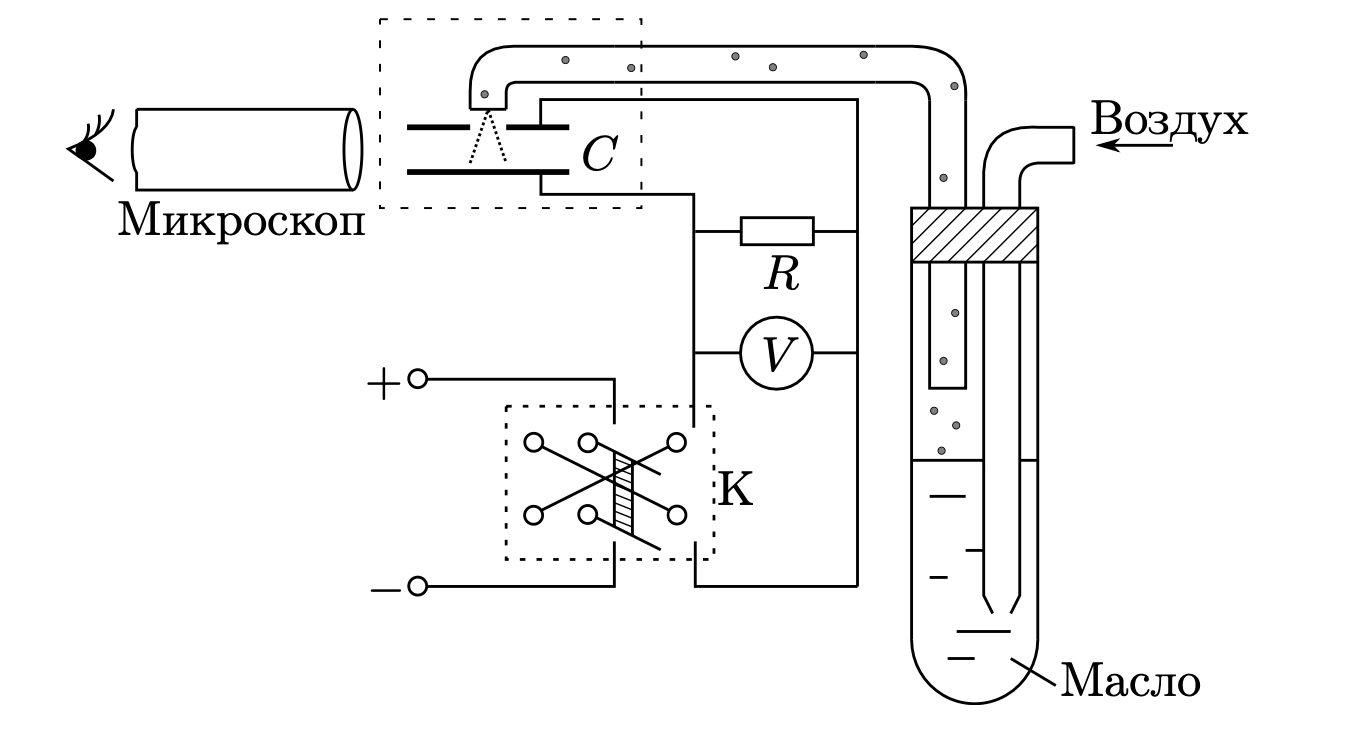
\includegraphics[width=0.8\linewidth]{Снимок экрана 2024-12-24 в 19.44.51.png}
    \caption{Схема установки}
    \label{fig:ustan}
\end{figure}
\noindent
Через маленькое отверстие верхней пластины конденсатора C разбрызгиваем капли масла. Из-за трения о воздух капли приобретают случайный по абсолютной величине и знаку электрический заряд.

Подаём на пластины конденсатора напряжение, которое будем измерять вольтметром V. Ключом К меняем направление поля в конденсаторе, чтобы можно было вернуть каплю на прежнее место и снова произвести измерение. В фокальной плоскости окуляра измерительного микроскопа виден ряд горизонтальных линий, расстояние между которыми равно 0.25 мм. Наблюдая за перемещением капли между линиями, можно определить пройденный каплей путь. Время t свободного падения капли от одной выбранной линии до другой и время t' её обратного подъёма, происходящего под действием сил электрического поля, измеряем секундомером. После размыкании ключа конденсатор разрядится через сопротивление R.
\newpage
\section{Теоретическое введение}
Существование элементарного заряда приводит к дискретности значений заряда $q$:
\begin{equation}
    q = 0, \pm e, \pm 2e, \pm 3e, ..., \pm ne ...,
\end{equation}

В данном опыте измеряется заряд малых капель масла, несущих несколько элементарных зарядов. Сравнив заряды между собой мы убедимся в их кратности элементарному заряду $e$.

\subsection*{Уравнение движения капли}
Рассмотрим свободное падение капли, применим второй закон Ньютона:

\begin{equation}
    m \frac{dv}{dt} = mg - F_{\text{тр}},
\end{equation}

При малых скоростях сила трения для сферической капли определяется формулой Стокса:

\begin{equation}
    F_{\text{тр}} = 6\pi\eta r v = kv,
    \label{eq:friction}
\end{equation}
где $r$ - радиус капли $\eta$ - коэффициент вязкости трения воздуха.
Подставляя (3) в (2) проинтегрируем уравнение по времени ($v_{0} = 0$), получим:

\begin{equation}
    v = v_{\infty}(1 - e^{-kt/m}),
    \label{eq:speed_inf}
\end{equation}

где $v_{\infty}$ - установившаяся скорость падения

\begin{equation}
    v_{\infty} = \frac{mg}{q}=\frac{\frac{4}{3} \pi \rho r^{3} g}{6 \pi \rho r}=\frac{2}{9}\frac{\rho}{\eta}g r^{2}.
    \label{eq:speed_inf_calculated}
\end{equation}

где $\rho$ - плотность масла. Согласно (4), установление скорости происходит за характерное время:

\begin{equation}
    \tau = \frac{m}{k}=\frac{v_{\infty}}{g} = \frac{2}{9}\frac{\rho}{\eta} r^{2}.
    \label{eq:tau}
\end{equation}

Из-за очень малого размера капли, можно считать, что её движение всегда равно \\ установившемуся.
\\
Тогда зная время падения капли. Определим её радиус, обозначим пройденный путь через $h \approx v_{\infty}t$:

\begin{equation}
    r = \sqrt{\frac{9 \eta h}{2 \rho gt} }.
    \label{eq:radius}
\end{equation}

Теперь рассмотрим движение капли при наличии электрического поля $E=U/l$. Если капля движется против $g$ то уравнение принимает вид:

\begin{equation}
    m\frac{dv}{dt} = \frac{qU}{l} - mg - kv,
\end{equation}

Дополнительная константа в правой части не изменяет постоянной времени $\theta = \frac{k}{m}$. Найдём новую установившуюся скорость, положим, что временем установления скорости можно пренебречь:

\begin{equation}
    v_{\infty}^{'} = \frac{qU}{kl} - v_{\infty},
    \label{eq:v_inf_real}
\end{equation}

пусть $t^{'} = h/v^{'}_{\infty}$ - время подъёма капли на начальную высоту. Используя равенства (\refeq{eq:friction}), (\refeq{eq:radius}) и (\refeq{eq:v_inf_real}), получим окончательную расчётную формулу для заряда капли:

\begin{equation}
    q = 9\pi \frac{l}{U} \sqrt{\frac{2}{\rho g}} (\eta h)^{3/2} \frac{t + t^{'}}{t^{3/2} t^{'}}.
    \label{eq:q_final}
\end{equation}

\subsection*{Оценка погрешности}

Дискретность заряда, можно определить если только погрешность измерения заряда много меньше элементарного заряда. Это условие легко выполнимо если кратность заряда - $n$ - мала. В условиях нашего опыта трудно произвести измерения с точностью лучше 5\%. Поэтому необходимо чтобы заряд капли был меньше $20e$ (оптимально — $5e$).

Проанализируем погрешность формулы (\refeq{eq:q_final}). Из всех велчин, входящих в формулу (\refeq{eq:q_final}), на опыте измеряются только $U, t, t^{'}$. Погрешность напряжения пренебрежимо мала, поэтому погрешность измерения $q$  определяется в основном погрешностью времени $\delta t$.

При визуальных наблюдениях фактором, определяющим величину погрешности , выступает время реакции человека, которое практически не бывает меньше $\delta t \approx 0,2$ с.

Из формулы (\refeq{eq:q_final}) нетрудно определить погрешность:

\begin{equation}
    \frac{\sigma_q}{q} = \sqrt{{\frac{\sigma^2_{U}}{U^{2}} + \frac{\sigma^2_{t} t_{0}^{2}}{t^{2} (t_{0}+t)^{2}}} + \frac{\sigma^2_{t_0}}{4t_{0}^{2}} \left(\frac{3 t + t_{0}}{t + t_{0}}\right)^{2}}
    \label{eq:q_deviation}
\end{equation}

Из соотношения (\refeq{eq:q_deviation}) следует, что погрешность будет минимальна, если
времена $t \text{ и } t^{'}$ — величины одного порядка. В этом случае для
погрешности определения заряда имеем

\begin{equation}
    \frac{\sigma_q}{q} = \sqrt{\frac{\sigma^2_{U}}{U^{2}} + \frac{\sigma^2_{t}}{4t_{0}^{2}} + \frac{\sigma^2_{t_0}}{t_{0}^{2}}}
    \label{eq:q_deviation_final}
\end{equation}

\newpage
\section{Обработка результатов измерений}
%Оценим с помощью формулы (10) минимальное напряжение $U_{min} = 300 \text{ В}$, такое напряжение нужно для подъёма капель, несущих 5 зарядов электрона на высоту h = 1 мм. Напряжения, меньше этого будут поднимать слишком сильно заряженные капли, что приведёт к неточности эксперимента и слишком большим погрешностям.
\noindent
\textbf{Условия эксперимента:}
\\
Расстояние между пластинами $l = 0.725$ см, плотность масла $\rho = 0.898 \,\, \text{г}/\text{см}^3$, вязкость воздуха $\eta = 1.85 \cdot 10^{-5} \, \text{Па} \cdot \text{с}$ ($T = 300$ К), цена деления окуляра $b = 0.25$ мм, $U_\text{min} = 300 \, \text{В}$.
\\
\textbf{Определение величины элементарного заряда:}
\\
Для 14 капель проведём измерение их зарядов $q$, результаты представлены в таблице:
\begin{table}[H]
    \centering
    \begin{tabular}{|c|c|c|c|c|c|c|}
        \hline
        $N_\text{зар}$ & $U_\text{конд}, \text{ В}$ & $t_0, \text{ с}$ & $t, \text{ с}$ & $q_\text{ср} \cdot 10^{-19}\text{ Кл}$ & $n_\text{шт}$ \\
        \hline
        1 & 300 & 32.68 & 9.59  & $(6.09   \pm 1.506)$ & 4    \\
        2 & 400 & 28.88 & 7.91  & $(5.81   \pm 1.245)$ & 4    \\
        3 & 400 & 26.48 & 8.06  & $(6.08   \pm 1.528)$ & 4    \\
        4 & 400 & 18.46 & 3.06  & $(17.17  \pm 3.163)$ & 10   \\
        5 & 400 & 16.11 & 3.39  & $(17.18  \pm 3.484)$ & 10   \\
        6 & 400 & 22.47 & 10.15 & $(5.83  \pm 0.923)$ & 4    \\
        7 & 400 & 26.26 & 9.05  & $(5.62   \pm 1.523)$ & 3    \\
        8 & 400 & 25.44 & 8.86  & $(5.87   \pm 1.531)$ & 4    \\
        9 & 400 & 21.69 & 10.33 & $(5.95  \pm 1.681)$ & 4    \\
        10 & 400 & 32.03 & 6.90 & $(6.03  \pm 1.530)$ & 4    \\
        11 & 400 & 24.04 & 3.77 & $(12.13 \pm 3.194)$ & 7    \\
        12 & 400 & 27.91 & 7.22 & $(6.40  \pm 1.827)$ & 4    \\
        13 & 400 & 8.72 & 7.20  & $(1.65   \pm 0.271)$ & 1    \\
        14 & 400 & 12.24 & 4.52 & $(16.72 \pm 3.531)$ & 10   \\
        \hline
    \end{tabular}
    \caption{Таблица с результатами измерений}
\end{table}

\begin{figure}[H]
    \centering
    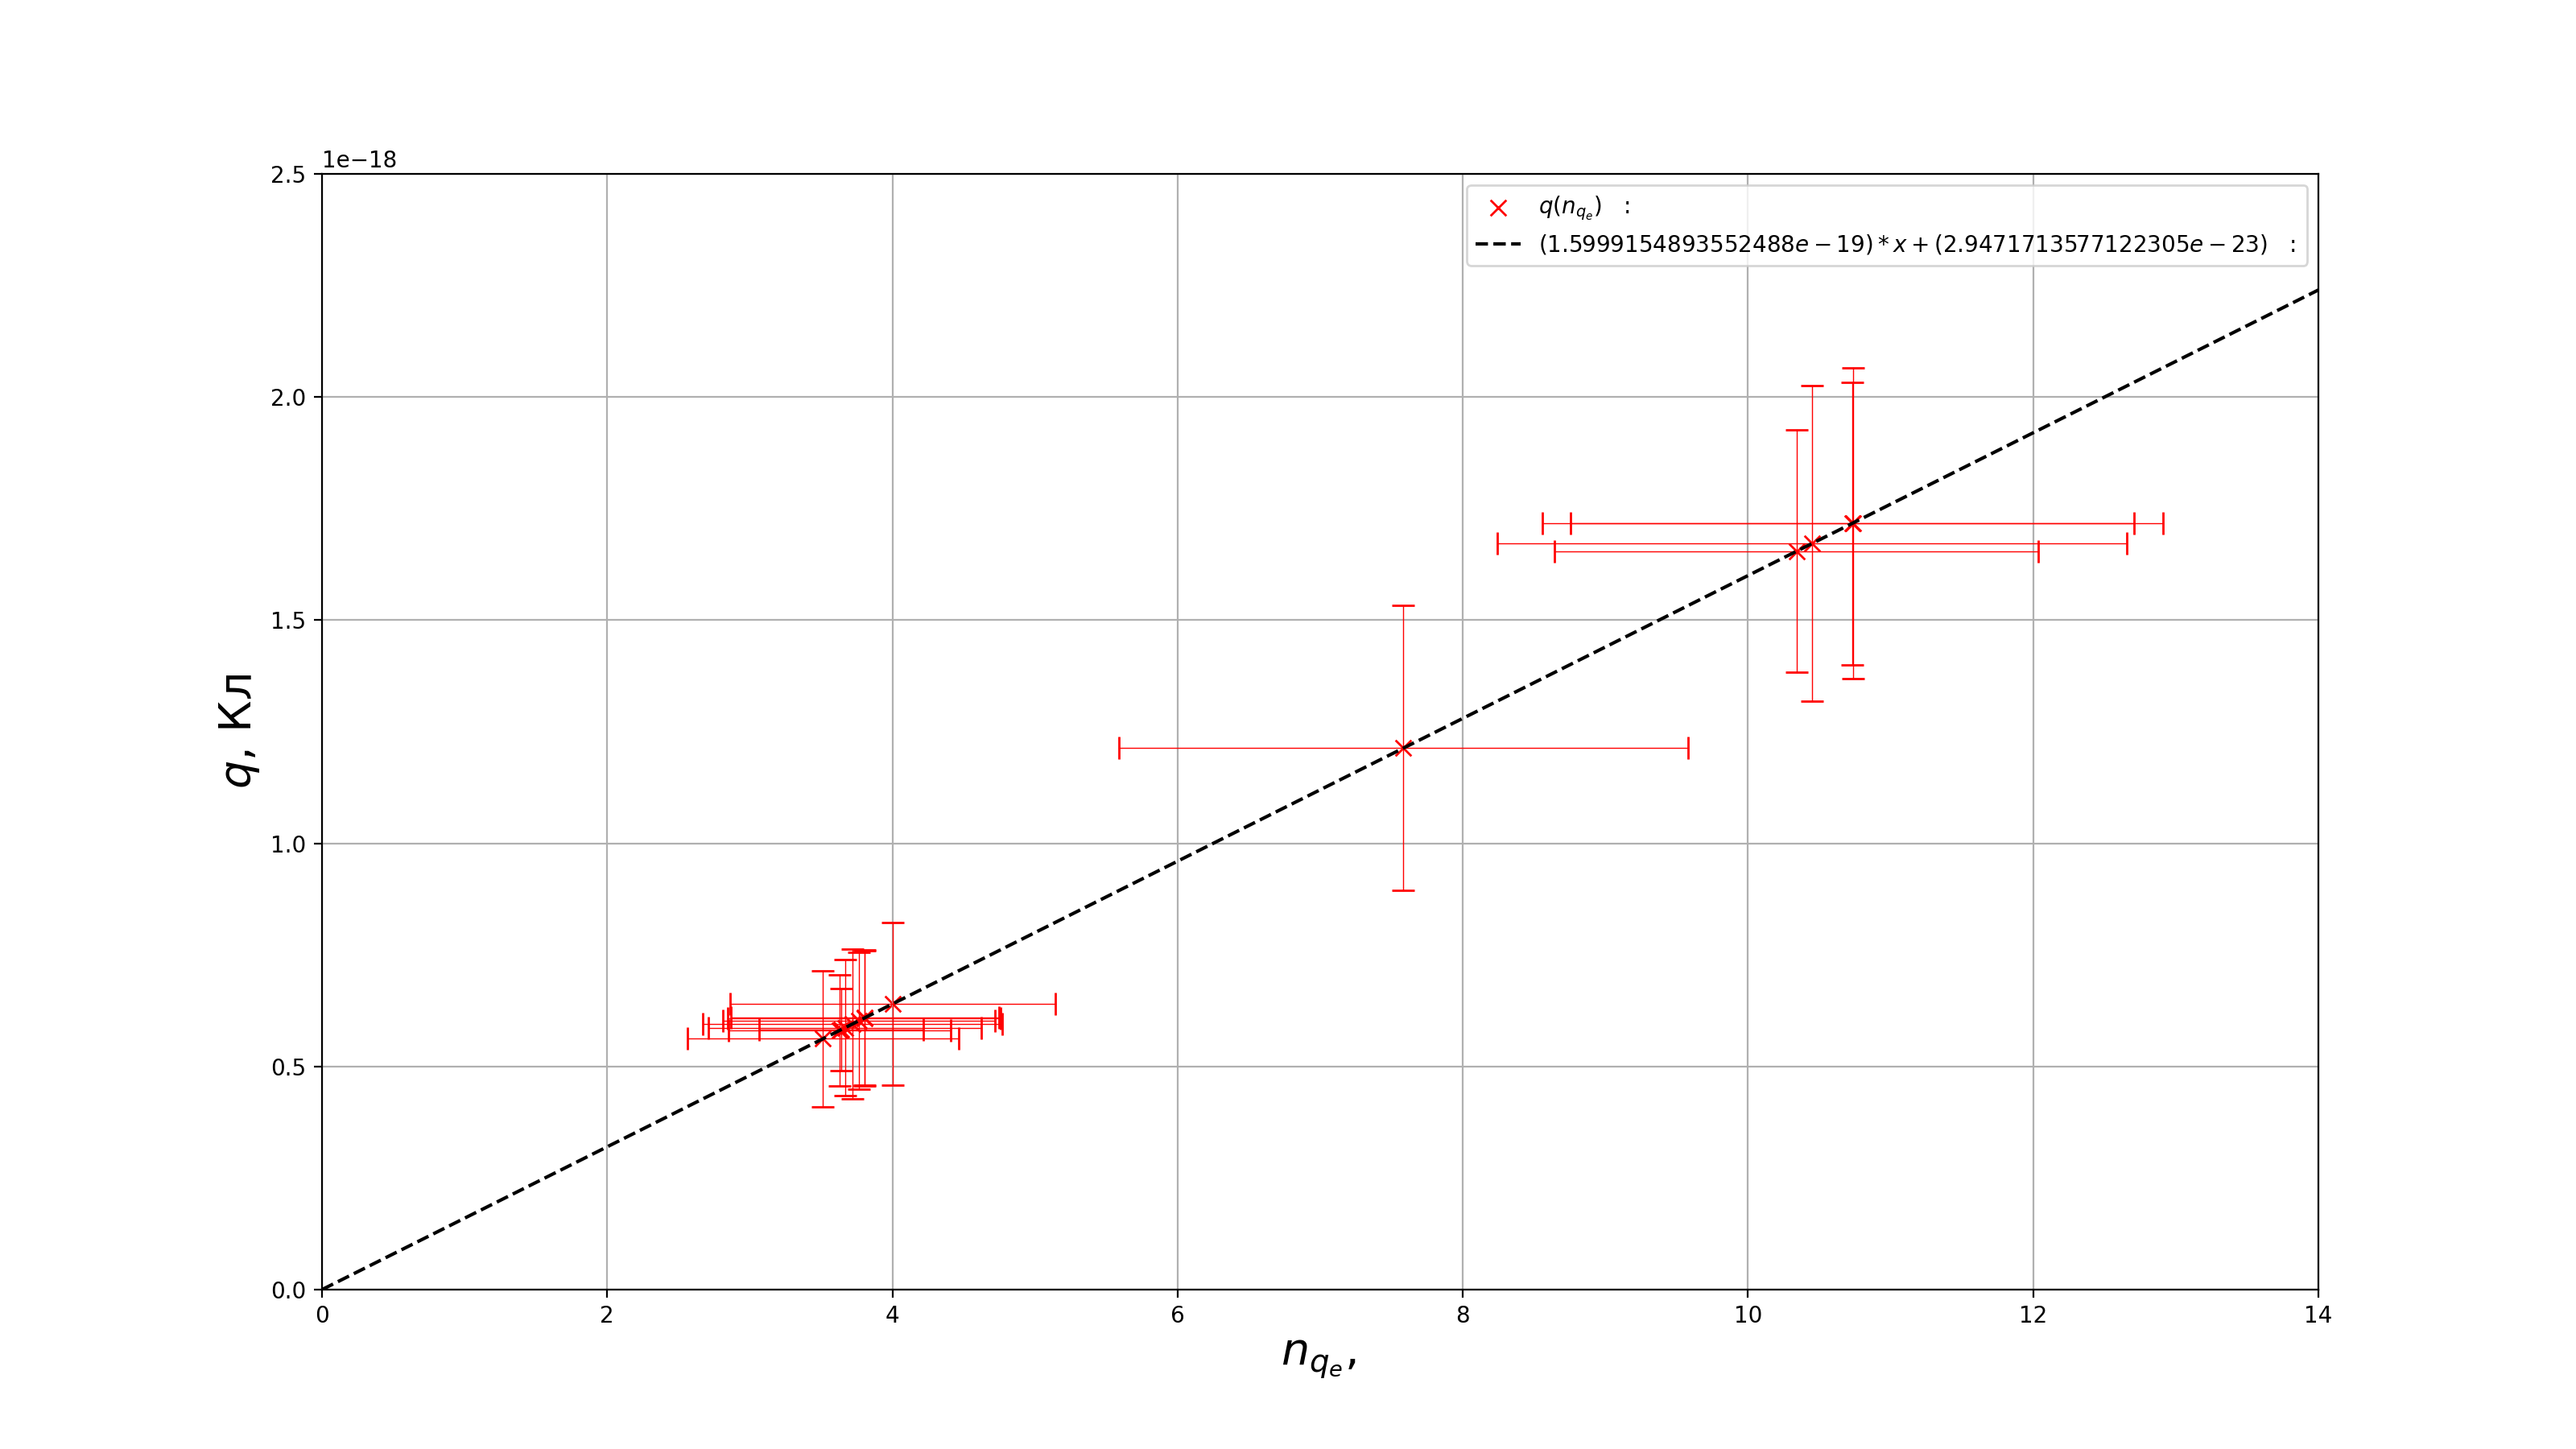
\includegraphics[width=\textwidth]{graph.png}
    \caption{График зависимости заряда капли масла от кол-ва элементарных зарядов}
    \label{graph:q_n}
\end{figure}

По наклону графика можно определить элементарный заряд электрона $|e^{-}| = (1.600 \pm 0.120) * 10^-19$ Кл.

\section{Сравнение с опытом Толмена}

Пусть в единице объёма металла $n$ свободных электронов. Так как движение зарядов хаотично и равновероятно, то их плотность тока равна 0. Пусть в какой-то момент возникло упорядоченное движение электронов со средней скоростью $u$. Тогда плотность возникшего тока через единицу площади равна:

\begin{equation}
    j = enu
\end{equation}

Рассмотрим неравномерное вращение металогического кольца вокруг своей оси (линейная скорость равна $v$). Если бы свободные электроны были крепко связанны с атомами и двигались совместно то движения положительных и отрицательных зарядов создавали бы токи равные и противоположно направленные, если же электроны были неподвижны то ток определялся бы только движением положительных зарядов:

\begin{equation}
    j = -env = enu
\end{equation}

Однако в действительности неравномерное движение кристаллической решётки увлекает за собой часть электронов, вследствие чего будет возникать переменный ток.
Уравнение движения электронов примет вид:

\begin{equation}
    m \frac{d}{dt} (v_{w} + u) = F
\end{equation}

где $(v_{w} + u)$ - полная скорость электрона, а $F$ - действующая на него сила. Характеризуемая столкновениями между электронами и решёткой характеризуемое сопротивлением металла $R$ и ЭДС индукции, сопротивляющаяся всякому изменению силы тока в проводнике характеризуемое индуктивностью металла $L$. Обе эти силы зависят от $u$ а не от полной скорости электронов, тогда получим:

\begin{equation}
    m \frac{du}{dt}  = F(u) - m \frac{dv_{w}}{dt}
\end{equation}

где последнее слагаемое представляет собой силу инерции относительно движущейся системы. Воспользуемся непосредственно общим уравнением переменных токов.

\begin{equation}
    \frac{1}{c}L\frac{dJ}{dt} +RI  = \oint{E^{\text{стр}}_{s}}dS,
\end{equation}

приравняв сторонней силе $ eE^{\text{стр}}_{s}$ силу инерции $\frac{dv_{w}}{dt}$ получим:

\begin{equation}
    \frac{1}{c}L\frac{dJ}{dt} +RI  = - \frac{m}{e} \oint{\frac{dv_{w}}{dt}}dS = - \frac{ms}{e} \frac{dv_{w}}{dt}
\end{equation}

где $s$ -длинна кольца. Проинтегрировав по времени получим от $t = t_1$ до $t = t_2$ пологая, что в эти промежутки ток обращается в 0.

\begin{equation}
    R\int_{t_2}^{t_1} J \,dt = - \frac{ms}{e} (v_{w}(t_2) - v_{w}(t_1))
\end{equation}

Этим соотношением Толмен воспользовался для определения отношения $e/m$ в металле. Круглая проволочная катушка приводилась в движение и затем (в момент времени $t_1$) тормозилась и приводилась в состояние покоя ($v_{w}(t_2) = 0$) в течение доли секунды. В течении этого промежутка времени по катушке тёк ток, измеряемый неподвижным гальванометром. Измерив $R\int_{t_2}^{t_1} J \,dt$ и $v_{w}(t_1)$ и учтя все все побочные эффекты, можно рассчитать отношение $m/e$ для носителей тока в металле.

полученное экспериментальное значение в опытах Толмена оказалось равным:

\begin{equation}
    m/e = 4,58 \cdot 10^{-9} \text{г/Кл} = 1,53 \cdot 10^{-18} \text{абс. ед. СГС,}
\end{equation}

\begin{equation}
    e = 1,986\cdot 10^{-19} \text{Кл}
\end{equation}

Что согласуется по порядку величины со значением полученным при измерениях над свободными электронами в катодных лучах

\begin{equation}
    m/e = 5,66 \cdot 10^{-9} \text{г/Кл}  = 1,9 \cdot 10^{-18} \text{абс. ед. СГС,}
\end{equation}

\begin{equation}
    e = 1,608\cdot 10^{-19} \text{Кл}
\end{equation}

\section{Вывод}
В данном опыте мы получили значение элементарного заряда методом Миллекена $e^{-} = 1.600 \cdot10^{-19} \text{ Кл}$, что в пределах погрешности сходится с теоретическим значением, сравнив с методом получения элементарного заряда по Толмену, мы пришли к выводу, что в нашей работе реальный заряд электрона $e^{-}$ определяется точнее, относительная погрешность в опыте Миллекена равняется 6\%, в опыте Толмена она равна 23.05 \%.
\end{document}

\end{document}